\documentclass[twoside]{book}

% Packages required by doxygen
\usepackage{fixltx2e}
\usepackage{calc}
\usepackage{doxygen}
\usepackage[export]{adjustbox} % also loads graphicx
\usepackage{graphicx}
\usepackage[utf8]{inputenc}
\usepackage{makeidx}
\usepackage{multicol}
\usepackage{multirow}
\PassOptionsToPackage{warn}{textcomp}
\usepackage{textcomp}
\usepackage[nointegrals]{wasysym}
\usepackage[table]{xcolor}

% Font selection
\usepackage[T1]{fontenc}
\usepackage[scaled=.90]{helvet}
\usepackage{courier}
\usepackage{amssymb}
\usepackage{sectsty}
\renewcommand{\familydefault}{\sfdefault}
\allsectionsfont{%
  \fontseries{bc}\selectfont%
  \color{darkgray}%
}
\renewcommand{\DoxyLabelFont}{%
  \fontseries{bc}\selectfont%
  \color{darkgray}%
}
\newcommand{\+}{\discretionary{\mbox{\scriptsize$\hookleftarrow$}}{}{}}

% Page & text layout
\usepackage{geometry}
\geometry{%
  a4paper,%
  top=2.5cm,%
  bottom=2.5cm,%
  left=2.5cm,%
  right=2.5cm%
}
\tolerance=750
\hfuzz=15pt
\hbadness=750
\setlength{\emergencystretch}{15pt}
\setlength{\parindent}{0cm}
\setlength{\parskip}{3ex plus 2ex minus 2ex}
\makeatletter
\renewcommand{\paragraph}{%
  \@startsection{paragraph}{4}{0ex}{-1.0ex}{1.0ex}{%
    \normalfont\normalsize\bfseries\SS@parafont%
  }%
}
\renewcommand{\subparagraph}{%
  \@startsection{subparagraph}{5}{0ex}{-1.0ex}{1.0ex}{%
    \normalfont\normalsize\bfseries\SS@subparafont%
  }%
}
\makeatother

% Headers & footers
\usepackage{fancyhdr}
\pagestyle{fancyplain}
\fancyhead[LE]{\fancyplain{}{\bfseries\thepage}}
\fancyhead[CE]{\fancyplain{}{}}
\fancyhead[RE]{\fancyplain{}{\bfseries\leftmark}}
\fancyhead[LO]{\fancyplain{}{\bfseries\rightmark}}
\fancyhead[CO]{\fancyplain{}{}}
\fancyhead[RO]{\fancyplain{}{\bfseries\thepage}}
\fancyfoot[LE]{\fancyplain{}{}}
\fancyfoot[CE]{\fancyplain{}{}}
\fancyfoot[RE]{\fancyplain{}{\bfseries\scriptsize Generated by Doxygen }}
\fancyfoot[LO]{\fancyplain{}{\bfseries\scriptsize Generated by Doxygen }}
\fancyfoot[CO]{\fancyplain{}{}}
\fancyfoot[RO]{\fancyplain{}{}}
\renewcommand{\footrulewidth}{0.4pt}
\renewcommand{\chaptermark}[1]{%
  \markboth{#1}{}%
}
\renewcommand{\sectionmark}[1]{%
  \markright{\thesection\ #1}%
}

% Indices & bibliography
\usepackage{natbib}
\usepackage[titles]{tocloft}
\setcounter{tocdepth}{3}
\setcounter{secnumdepth}{5}
\makeindex

% Hyperlinks (required, but should be loaded last)
\usepackage{ifpdf}
\ifpdf
  \usepackage[pdftex,pagebackref=true]{hyperref}
\else
  \usepackage[ps2pdf,pagebackref=true]{hyperref}
\fi
\hypersetup{%
  colorlinks=true,%
  linkcolor=blue,%
  citecolor=blue,%
  unicode%
}

% Custom commands
\newcommand{\clearemptydoublepage}{%
  \newpage{\pagestyle{empty}\cleardoublepage}%
}

\usepackage{caption}
\captionsetup{labelsep=space,justification=centering,font={bf},singlelinecheck=off,skip=4pt,position=top}

%===== C O N T E N T S =====

\begin{document}

% Titlepage & ToC
\hypersetup{pageanchor=false,
             bookmarksnumbered=true,
             pdfencoding=unicode
            }
\pagenumbering{alph}
\begin{titlepage}
\vspace*{7cm}
\begin{center}%
{\Large Reusabili\+Token\+Simulator \\[1ex]\large v1 }\\
\vspace*{1cm}
{\large Generated by Doxygen 1.8.14}\\
\end{center}
\end{titlepage}
\clearemptydoublepage
\pagenumbering{roman}
\tableofcontents
\clearemptydoublepage
\pagenumbering{arabic}
\hypersetup{pageanchor=true}

%--- Begin generated contents ---
\chapter{Namespace Index}
\section{Packages}
Here are the packages with brief descriptions (if available)\+:\begin{DoxyCompactList}
\item\contentsline{section}{\mbox{\hyperlink{namespaceapp__reusability_token__simulator}{app\+\_\+reusability\+Token\+\_\+simulator}} }{\pageref{namespaceapp__reusability_token__simulator}}{}
\item\contentsline{section}{\mbox{\hyperlink{namespace_customer}{Customer}} }{\pageref{namespace_customer}}{}
\item\contentsline{section}{\mbox{\hyperlink{namespace_shop}{Shop}} }{\pageref{namespace_shop}}{}
\item\contentsline{section}{\mbox{\hyperlink{namespace_shop_list_oracle}{Shop\+List\+Oracle}} }{\pageref{namespace_shop_list_oracle}}{}
\item\contentsline{section}{\mbox{\hyperlink{namespace_simulation_engine}{Simulation\+Engine}} }{\pageref{namespace_simulation_engine}}{}
\item\contentsline{section}{\mbox{\hyperlink{namespace_simulation_time_oracle}{Simulation\+Time\+Oracle}} }{\pageref{namespace_simulation_time_oracle}}{}
\item\contentsline{section}{\mbox{\hyperlink{namespace_smart_contract}{Smart\+Contract}} }{\pageref{namespace_smart_contract}}{}
\item\contentsline{section}{\mbox{\hyperlink{namespace_visualization}{Visualization}} }{\pageref{namespace_visualization}}{}
\end{DoxyCompactList}

\chapter{Hierarchical Index}
\section{Class Hierarchy}
This inheritance list is sorted roughly, but not completely, alphabetically\+:\begin{DoxyCompactList}
\item object\begin{DoxyCompactList}
\item \contentsline{section}{Customer.\+Customer}{\pageref{class_customer_1_1_customer}}{}
\begin{DoxyCompactList}
\item \contentsline{section}{Customer.\+Bad\+Customer}{\pageref{class_customer_1_1_bad_customer}}{}
\item \contentsline{section}{Customer.\+Good\+Customer}{\pageref{class_customer_1_1_good_customer}}{}
\item \contentsline{section}{Customer.\+Neutral\+Customer}{\pageref{class_customer_1_1_neutral_customer}}{}
\end{DoxyCompactList}
\item \contentsline{section}{Shop.\+Shop}{\pageref{class_shop_1_1_shop}}{}
\item \contentsline{section}{Shop\+List\+Oracle.\+Shop\+List\+Oracle}{\pageref{class_shop_list_oracle_1_1_shop_list_oracle}}{}
\item \contentsline{section}{Simulation\+Engine.\+Simulation\+Engine}{\pageref{class_simulation_engine_1_1_simulation_engine}}{}
\item \contentsline{section}{Simulation\+Time\+Oracle.\+Simulation\+Time\+Oracle}{\pageref{class_simulation_time_oracle_1_1_simulation_time_oracle}}{}
\item \contentsline{section}{Smart\+Contract.\+Smart\+Contract}{\pageref{class_smart_contract_1_1_smart_contract}}{}
\end{DoxyCompactList}
\end{DoxyCompactList}

\chapter{Class Index}
\section{Class List}
Here are the classes, structs, unions and interfaces with brief descriptions\+:\begin{DoxyCompactList}
\item\contentsline{section}{\mbox{\hyperlink{class_customer_1_1_bad_customer}{Customer.\+Bad\+Customer}} }{\pageref{class_customer_1_1_bad_customer}}{}
\item\contentsline{section}{\mbox{\hyperlink{class_customer_1_1_customer}{Customer.\+Customer}} }{\pageref{class_customer_1_1_customer}}{}
\item\contentsline{section}{\mbox{\hyperlink{class_customer_1_1_good_customer}{Customer.\+Good\+Customer}} }{\pageref{class_customer_1_1_good_customer}}{}
\item\contentsline{section}{\mbox{\hyperlink{class_customer_1_1_neutral_customer}{Customer.\+Neutral\+Customer}} }{\pageref{class_customer_1_1_neutral_customer}}{}
\item\contentsline{section}{\mbox{\hyperlink{class_shop_1_1_shop}{Shop.\+Shop}} }{\pageref{class_shop_1_1_shop}}{}
\item\contentsline{section}{\mbox{\hyperlink{class_shop_list_oracle_1_1_shop_list_oracle}{Shop\+List\+Oracle.\+Shop\+List\+Oracle}} }{\pageref{class_shop_list_oracle_1_1_shop_list_oracle}}{}
\item\contentsline{section}{\mbox{\hyperlink{class_simulation_engine_1_1_simulation_engine}{Simulation\+Engine.\+Simulation\+Engine}} }{\pageref{class_simulation_engine_1_1_simulation_engine}}{}
\item\contentsline{section}{\mbox{\hyperlink{class_simulation_time_oracle_1_1_simulation_time_oracle}{Simulation\+Time\+Oracle.\+Simulation\+Time\+Oracle}} }{\pageref{class_simulation_time_oracle_1_1_simulation_time_oracle}}{}
\item\contentsline{section}{\mbox{\hyperlink{class_smart_contract_1_1_smart_contract}{Smart\+Contract.\+Smart\+Contract}} }{\pageref{class_smart_contract_1_1_smart_contract}}{}
\end{DoxyCompactList}

\chapter{Namespace Documentation}
\hypertarget{namespaceapp__reusability_token__simulator}{}\section{app\+\_\+reusability\+Token\+\_\+simulator Namespace Reference}
\label{namespaceapp__reusability_token__simulator}\index{app\+\_\+reusability\+Token\+\_\+simulator@{app\+\_\+reusability\+Token\+\_\+simulator}}
\subsection*{Functions}
\begin{DoxyCompactItemize}
\item 
\mbox{\Hypertarget{namespaceapp__reusability_token__simulator_ad7c965ffa90c952ccc9d4a5d38d89d82}\label{namespaceapp__reusability_token__simulator_ad7c965ffa90c952ccc9d4a5d38d89d82}} 
def {\bfseries setup\+\_\+args} ()
\item 
\mbox{\Hypertarget{namespaceapp__reusability_token__simulator_a9076ad1236189e798219334d36b9ae2a}\label{namespaceapp__reusability_token__simulator_a9076ad1236189e798219334d36b9ae2a}} 
def {\bfseries run\+\_\+simulator} ()
\end{DoxyCompactItemize}
\subsection*{Variables}
\begin{DoxyCompactItemize}
\item 
\mbox{\Hypertarget{namespaceapp__reusability_token__simulator_addc9601ebae0635bff3008f214ffeddc}\label{namespaceapp__reusability_token__simulator_addc9601ebae0635bff3008f214ffeddc}} 
int {\bfseries num\+\_\+iterations} = 100
\item 
\mbox{\Hypertarget{namespaceapp__reusability_token__simulator_a0c869441de9440494fa9c97da0c28d1e}\label{namespaceapp__reusability_token__simulator_a0c869441de9440494fa9c97da0c28d1e}} 
int {\bfseries num\+\_\+customers} = 3
\item 
\mbox{\Hypertarget{namespaceapp__reusability_token__simulator_abe6c8679105665a2d9602e97c8688699}\label{namespaceapp__reusability_token__simulator_abe6c8679105665a2d9602e97c8688699}} 
int {\bfseries num\+\_\+shops} = 2
\end{DoxyCompactItemize}


\subsection{Detailed Description}
\begin{DoxyVerb}@package app_reusabilityToken_simulator
Simulates a market where reusability tokens are at work

For usage: python app_reusabilityToken_simulator.py --help
\end{DoxyVerb}
 
\hypertarget{namespace_customer}{}\section{Customer Namespace Reference}
\label{namespace_customer}\index{Customer@{Customer}}
\subsection*{Classes}
\begin{DoxyCompactItemize}
\item 
class \mbox{\hyperlink{class_customer_1_1_bad_customer}{Bad\+Customer}}
\item 
class \mbox{\hyperlink{class_customer_1_1_customer}{Customer}}
\item 
class \mbox{\hyperlink{class_customer_1_1_good_customer}{Good\+Customer}}
\item 
class \mbox{\hyperlink{class_customer_1_1_neutral_customer}{Neutral\+Customer}}
\end{DoxyCompactItemize}


\subsection{Detailed Description}
\begin{DoxyVerb}@package Customer
Implementation of a generic Customer
\end{DoxyVerb}
 
\hypertarget{namespace_shop}{}\section{Shop Namespace Reference}
\label{namespace_shop}\index{Shop@{Shop}}
\subsection*{Classes}
\begin{DoxyCompactItemize}
\item 
class \mbox{\hyperlink{class_shop_1_1_shop}{Shop}}
\end{DoxyCompactItemize}


\subsection{Detailed Description}
\begin{DoxyVerb}@package Shop
Implementation of a shop
\end{DoxyVerb}
 
\hypertarget{namespace_shop_list_oracle}{}\section{Shop\+List\+Oracle Namespace Reference}
\label{namespace_shop_list_oracle}\index{Shop\+List\+Oracle@{Shop\+List\+Oracle}}
\subsection*{Classes}
\begin{DoxyCompactItemize}
\item 
class \mbox{\hyperlink{class_shop_list_oracle_1_1_shop_list_oracle}{Shop\+List\+Oracle}}
\end{DoxyCompactItemize}


\subsection{Detailed Description}
\begin{DoxyVerb}@package ShopListOracle
Implementation of a simple shop list oracle
\end{DoxyVerb}
 
\hypertarget{namespace_simulation_engine}{}\section{Simulation\+Engine Namespace Reference}
\label{namespace_simulation_engine}\index{Simulation\+Engine@{Simulation\+Engine}}
\subsection*{Classes}
\begin{DoxyCompactItemize}
\item 
class \mbox{\hyperlink{class_simulation_engine_1_1_simulation_engine}{Simulation\+Engine}}
\end{DoxyCompactItemize}


\subsection{Detailed Description}
\begin{DoxyVerb}@package SimulationEngine
Implementation of a simulation Engine
\end{DoxyVerb}
 
\hypertarget{namespace_simulation_time_oracle}{}\section{Simulation\+Time\+Oracle Namespace Reference}
\label{namespace_simulation_time_oracle}\index{Simulation\+Time\+Oracle@{Simulation\+Time\+Oracle}}
\subsection*{Classes}
\begin{DoxyCompactItemize}
\item 
class \mbox{\hyperlink{class_simulation_time_oracle_1_1_simulation_time_oracle}{Simulation\+Time\+Oracle}}
\end{DoxyCompactItemize}


\subsection{Detailed Description}
\begin{DoxyVerb}@package SimulationTimeOracle
Implementation of a timing oracle
\end{DoxyVerb}
 
\hypertarget{namespace_smart_contract}{}\section{Smart\+Contract Namespace Reference}
\label{namespace_smart_contract}\index{Smart\+Contract@{Smart\+Contract}}
\subsection*{Classes}
\begin{DoxyCompactItemize}
\item 
class \mbox{\hyperlink{class_smart_contract_1_1_smart_contract}{Smart\+Contract}}
\end{DoxyCompactItemize}


\subsection{Detailed Description}
\begin{DoxyVerb}@package SmartContract
Implementation of a smart contract
\end{DoxyVerb}
 
\hypertarget{namespace_visualization}{}\section{Visualization Namespace Reference}
\label{namespace_visualization}\index{Visualization@{Visualization}}
\subsection*{Functions}
\begin{DoxyCompactItemize}
\item 
def \mbox{\hyperlink{namespace_visualization_a6e47cd3e3c863758dc8c30a9f27330f0}{visualize\+\_\+function}} (values, name, color, ax=None)
\item 
def \mbox{\hyperlink{namespace_visualization_a293d9622a724c53c2d8d3e09bb9721c6}{visualize\+\_\+market}} (smart\+\_\+contract, customer\+\_\+list, shop\+\_\+list, ax\+\_\+cus=None, ax\+\_\+shop=None, ax\+\_\+cp=None, ax\+\_\+ca=None)
\item 
def \mbox{\hyperlink{namespace_visualization_a02f7aadcda80e9aca64ca6aeb1843803}{diminishing\+\_\+returns}} (max\+\_\+val, b1, num\+\_\+samples=100)
\end{DoxyCompactItemize}


\subsection{Detailed Description}
\begin{DoxyVerb}@package Visualization
Implementation of a few visualizers
\end{DoxyVerb}
 

\subsection{Function Documentation}
\mbox{\Hypertarget{namespace_visualization_a02f7aadcda80e9aca64ca6aeb1843803}\label{namespace_visualization_a02f7aadcda80e9aca64ca6aeb1843803}} 
\index{Visualization@{Visualization}!diminishing\+\_\+returns@{diminishing\+\_\+returns}}
\index{diminishing\+\_\+returns@{diminishing\+\_\+returns}!Visualization@{Visualization}}
\subsubsection{\texorpdfstring{diminishing\+\_\+returns()}{diminishing\_returns()}}
{\footnotesize\ttfamily def Visualization.\+diminishing\+\_\+returns (\begin{DoxyParamCaption}\item[{}]{max\+\_\+val,  }\item[{}]{b1,  }\item[{}]{num\+\_\+samples = {\ttfamily 100} }\end{DoxyParamCaption})}

\begin{DoxyVerb}Test function that generates values from a diminishing returns function
:param max_val: function cap
:param b1:0 >= some value <= 1
:param num_samples: the number of values to generate
:return: function values
\end{DoxyVerb}
 \mbox{\Hypertarget{namespace_visualization_a6e47cd3e3c863758dc8c30a9f27330f0}\label{namespace_visualization_a6e47cd3e3c863758dc8c30a9f27330f0}} 
\index{Visualization@{Visualization}!visualize\+\_\+function@{visualize\+\_\+function}}
\index{visualize\+\_\+function@{visualize\+\_\+function}!Visualization@{Visualization}}
\subsubsection{\texorpdfstring{visualize\+\_\+function()}{visualize\_function()}}
{\footnotesize\ttfamily def Visualization.\+visualize\+\_\+function (\begin{DoxyParamCaption}\item[{}]{values,  }\item[{}]{name,  }\item[{}]{color,  }\item[{}]{ax = {\ttfamily None} }\end{DoxyParamCaption})}

\begin{DoxyVerb}plot a function
:param values: function values
:param name: name of the function
:param color: color of te plot
:param ax: the axis on which to plot
:return: plot axis
\end{DoxyVerb}
 \mbox{\Hypertarget{namespace_visualization_a293d9622a724c53c2d8d3e09bb9721c6}\label{namespace_visualization_a293d9622a724c53c2d8d3e09bb9721c6}} 
\index{Visualization@{Visualization}!visualize\+\_\+market@{visualize\+\_\+market}}
\index{visualize\+\_\+market@{visualize\+\_\+market}!Visualization@{Visualization}}
\subsubsection{\texorpdfstring{visualize\+\_\+market()}{visualize\_market()}}
{\footnotesize\ttfamily def Visualization.\+visualize\+\_\+market (\begin{DoxyParamCaption}\item[{}]{smart\+\_\+contract,  }\item[{}]{customer\+\_\+list,  }\item[{}]{shop\+\_\+list,  }\item[{}]{ax\+\_\+cus = {\ttfamily None},  }\item[{}]{ax\+\_\+shop = {\ttfamily None},  }\item[{}]{ax\+\_\+cp = {\ttfamily None},  }\item[{}]{ax\+\_\+ca = {\ttfamily None} }\end{DoxyParamCaption})}

\begin{DoxyVerb}Function the visualizes the market
:param smart_contract: the smart contract containing the state of the block chain
:param customer_list: a list of customers in the block chain
:param shop_list: a list of shops in the block chain
:param ax_cus: the axis on which we plot the cumulative customer reputation
:param ax_shop: the axis on which we plot the cumulative shop reputation
:param ax_cp: the axis on which we plot the number of times a customer spent a coin
:param ax_ca: the axis on which cumulative shop coin count
:return: plot axes
\end{DoxyVerb}
 
\chapter{Class Documentation}
\hypertarget{class_customer_1_1_bad_customer}{}\section{Customer.\+Bad\+Customer Class Reference}
\label{class_customer_1_1_bad_customer}\index{Customer.\+Bad\+Customer@{Customer.\+Bad\+Customer}}


Inheritance diagram for Customer.\+Bad\+Customer\+:\nopagebreak
\begin{figure}[H]
\begin{center}
\leavevmode
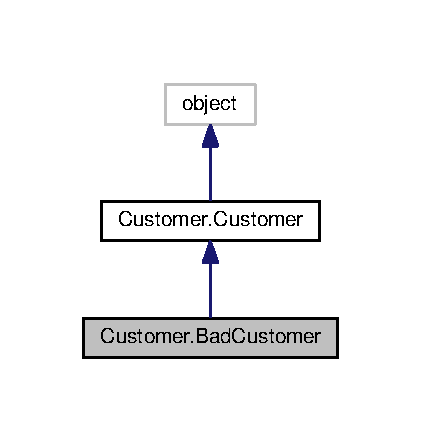
\includegraphics[width=202pt]{class_customer_1_1_bad_customer__inherit__graph}
\end{center}
\end{figure}


Collaboration diagram for Customer.\+Bad\+Customer\+:\nopagebreak
\begin{figure}[H]
\begin{center}
\leavevmode
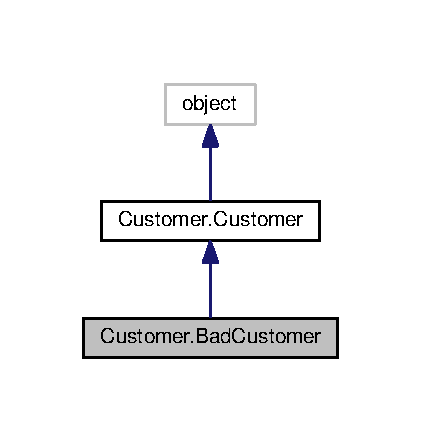
\includegraphics[width=202pt]{class_customer_1_1_bad_customer__coll__graph}
\end{center}
\end{figure}
\subsection*{Public Member Functions}
\begin{DoxyCompactItemize}
\item 
\mbox{\Hypertarget{class_customer_1_1_bad_customer_a5fb1dbd2f1cb6d0f89b61dcc197c22e4}\label{class_customer_1_1_bad_customer_a5fb1dbd2f1cb6d0f89b61dcc197c22e4}} 
def {\bfseries \+\_\+\+\_\+init\+\_\+\+\_\+} (self)
\item 
\mbox{\Hypertarget{class_customer_1_1_bad_customer_a95e7c9c31b4bd91ee0dafdf3c77c4485}\label{class_customer_1_1_bad_customer_a95e7c9c31b4bd91ee0dafdf3c77c4485}} 
def {\bfseries choose\+\_\+shop} (self, num\+\_\+shops)
\end{DoxyCompactItemize}
\subsection*{Public Attributes}
\begin{DoxyCompactItemize}
\item 
\mbox{\Hypertarget{class_customer_1_1_bad_customer_aed23368f8701a3693f8f9eaf1b734233}\label{class_customer_1_1_bad_customer_aed23368f8701a3693f8f9eaf1b734233}} 
{\bfseries recycle\+\_\+prob}
\end{DoxyCompactItemize}
\subsection*{Additional Inherited Members}


\subsection{Detailed Description}
\begin{DoxyVerb}A bad customer recycles goods with a very low probability and always visits stores in an erratic
fashion
\end{DoxyVerb}
 

The documentation for this class was generated from the following file\+:\begin{DoxyCompactItemize}
\item 
/home/prash/workspace/dev\+\_\+space/demo\+\_\+apps/\+Reusabili\+Token/\+Reusabili\+Token\+Simulator/src/Customer.\+py\end{DoxyCompactItemize}

\hypertarget{class_customer_1_1_customer}{}\section{Customer.\+Customer Class Reference}
\label{class_customer_1_1_customer}\index{Customer.\+Customer@{Customer.\+Customer}}


Inheritance diagram for Customer.\+Customer\+:\nopagebreak
\begin{figure}[H]
\begin{center}
\leavevmode
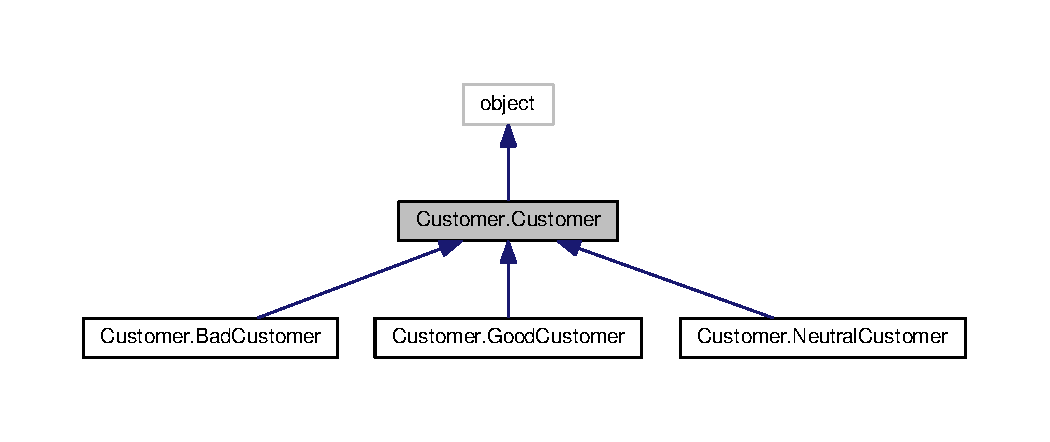
\includegraphics[width=350pt]{class_customer_1_1_customer__inherit__graph}
\end{center}
\end{figure}


Collaboration diagram for Customer.\+Customer\+:\nopagebreak
\begin{figure}[H]
\begin{center}
\leavevmode
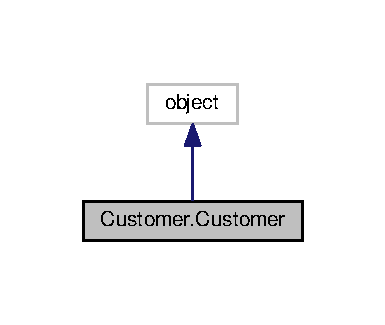
\includegraphics[width=185pt]{class_customer_1_1_customer__coll__graph}
\end{center}
\end{figure}
\subsection*{Public Member Functions}
\begin{DoxyCompactItemize}
\item 
\mbox{\Hypertarget{class_customer_1_1_customer_a448ae44d7fd2fecfff3bcaa607c0611a}\label{class_customer_1_1_customer_a448ae44d7fd2fecfff3bcaa607c0611a}} 
def {\bfseries \+\_\+\+\_\+init\+\_\+\+\_\+} (self, type\+\_\+)
\item 
def \mbox{\hyperlink{class_customer_1_1_customer_ace618f142ffda53d5538c0f354a0457a}{transfer\+\_\+coin}} (self, coin\+\_\+count)
\item 
def \mbox{\hyperlink{class_customer_1_1_customer_a61ab0c880d31a2f0d87d71f9d708ca45}{set\+\_\+coin}} (self, coins)
\item 
def \mbox{\hyperlink{class_customer_1_1_customer_a36bf1ca43a67bf563793e1ad7558711f}{transfer\+\_\+reputation}} (self, reputation, shop\+\_\+address)
\item 
def \mbox{\hyperlink{class_customer_1_1_customer_a7179b6123d3b732082c5724e7d416ab3}{set\+\_\+reputation}} (self, shop\+\_\+address, reputation)
\item 
def \mbox{\hyperlink{class_customer_1_1_customer_a77531667290ff6b0c5547ebf17930098}{get\+\_\+address}} (self)
\item 
def \mbox{\hyperlink{class_customer_1_1_customer_aecee1601bb165a1a341d65c2041a3cbf}{choose\+\_\+to\+\_\+recycle}} (self)
\item 
def \mbox{\hyperlink{class_customer_1_1_customer_a86df6d77038d58a8497b0dbcdb0d3872}{choose\+\_\+to\+\_\+pay\+\_\+by\+\_\+coin}} (self)
\item 
def \mbox{\hyperlink{class_customer_1_1_customer_a4c3a13a45a42e3179d30c75ccde32ec3}{get\+\_\+coin\+\_\+spend}} (self)
\item 
def \mbox{\hyperlink{class_customer_1_1_customer_a132ab8cbc2cdf93767fd1e7f295636c2}{get\+\_\+coin}} (self)
\item 
def \mbox{\hyperlink{class_customer_1_1_customer_a6053111a21363f88cbd7f296342d450d}{get\+\_\+reputation}} (self, shop\+\_\+address)
\item 
def \mbox{\hyperlink{class_customer_1_1_customer_afde17ca03b3a788bf821f3fa0309fd55}{get\+\_\+type}} (self)
\item 
def \mbox{\hyperlink{class_customer_1_1_customer_a38dfeb79b9aaa0e75bd78f3a5e23e71e}{choose\+\_\+shop}} (self, num\+\_\+shops)
\end{DoxyCompactItemize}
\subsection*{Public Attributes}
\begin{DoxyCompactItemize}
\item 
\mbox{\Hypertarget{class_customer_1_1_customer_aab3ad437a6d6d65d52a5a1876ba55132}\label{class_customer_1_1_customer_aab3ad437a6d6d65d52a5a1876ba55132}} 
{\bfseries customer\+\_\+id}
\item 
\mbox{\Hypertarget{class_customer_1_1_customer_a7a1bf903055ef024dfcce238793cc76f}\label{class_customer_1_1_customer_a7a1bf903055ef024dfcce238793cc76f}} 
{\bfseries reputation}
\item 
\mbox{\Hypertarget{class_customer_1_1_customer_a59e00114c437f593fe212790ddd55427}\label{class_customer_1_1_customer_a59e00114c437f593fe212790ddd55427}} 
{\bfseries coins}
\item 
\mbox{\Hypertarget{class_customer_1_1_customer_afeb97ca795d191873b7f27e41fab51a8}\label{class_customer_1_1_customer_afeb97ca795d191873b7f27e41fab51a8}} 
{\bfseries recycle\+\_\+prob}
\item 
\mbox{\Hypertarget{class_customer_1_1_customer_a9e378cb96ffdae61f782c87af9a624a1}\label{class_customer_1_1_customer_a9e378cb96ffdae61f782c87af9a624a1}} 
{\bfseries preferred\+\_\+shop}
\item 
\mbox{\Hypertarget{class_customer_1_1_customer_acfb18b95ddf55e0606859f23b033b0d1}\label{class_customer_1_1_customer_acfb18b95ddf55e0606859f23b033b0d1}} 
{\bfseries type\+\_\+}
\end{DoxyCompactItemize}
\subsection*{Static Public Attributes}
\begin{DoxyCompactItemize}
\item 
\mbox{\Hypertarget{class_customer_1_1_customer_a586cec6760e6de897c1c1b692fb24c0e}\label{class_customer_1_1_customer_a586cec6760e6de897c1c1b692fb24c0e}} 
int {\bfseries C\+U\+S\+T\+O\+M\+E\+R\+\_\+\+ID} = 0
\end{DoxyCompactItemize}


\subsection{Detailed Description}
\begin{DoxyVerb}This is a generic Customer class
\end{DoxyVerb}
 

\subsection{Member Function Documentation}
\mbox{\Hypertarget{class_customer_1_1_customer_a38dfeb79b9aaa0e75bd78f3a5e23e71e}\label{class_customer_1_1_customer_a38dfeb79b9aaa0e75bd78f3a5e23e71e}} 
\index{Customer\+::\+Customer@{Customer\+::\+Customer}!choose\+\_\+shop@{choose\+\_\+shop}}
\index{choose\+\_\+shop@{choose\+\_\+shop}!Customer\+::\+Customer@{Customer\+::\+Customer}}
\subsubsection{\texorpdfstring{choose\+\_\+shop()}{choose\_shop()}}
{\footnotesize\ttfamily def Customer.\+Customer.\+choose\+\_\+shop (\begin{DoxyParamCaption}\item[{}]{self,  }\item[{}]{num\+\_\+shops }\end{DoxyParamCaption})}

\begin{DoxyVerb}A choose shop strategy that depends on what type of a customer one is.
:param num_shops: The total number of shops available
:return: The chosen shop index
\end{DoxyVerb}
 \mbox{\Hypertarget{class_customer_1_1_customer_a86df6d77038d58a8497b0dbcdb0d3872}\label{class_customer_1_1_customer_a86df6d77038d58a8497b0dbcdb0d3872}} 
\index{Customer\+::\+Customer@{Customer\+::\+Customer}!choose\+\_\+to\+\_\+pay\+\_\+by\+\_\+coin@{choose\+\_\+to\+\_\+pay\+\_\+by\+\_\+coin}}
\index{choose\+\_\+to\+\_\+pay\+\_\+by\+\_\+coin@{choose\+\_\+to\+\_\+pay\+\_\+by\+\_\+coin}!Customer\+::\+Customer@{Customer\+::\+Customer}}
\subsubsection{\texorpdfstring{choose\+\_\+to\+\_\+pay\+\_\+by\+\_\+coin()}{choose\_to\_pay\_by\_coin()}}
{\footnotesize\ttfamily def Customer.\+Customer.\+choose\+\_\+to\+\_\+pay\+\_\+by\+\_\+coin (\begin{DoxyParamCaption}\item[{}]{self }\end{DoxyParamCaption})}

\begin{DoxyVerb}Takes a decision on whether this customer buys something with the coins he has
at a given instance in time.
:return: boolean flag indicating the customer's decision to buy with ReusabiliTokens
\end{DoxyVerb}
 \mbox{\Hypertarget{class_customer_1_1_customer_aecee1601bb165a1a341d65c2041a3cbf}\label{class_customer_1_1_customer_aecee1601bb165a1a341d65c2041a3cbf}} 
\index{Customer\+::\+Customer@{Customer\+::\+Customer}!choose\+\_\+to\+\_\+recycle@{choose\+\_\+to\+\_\+recycle}}
\index{choose\+\_\+to\+\_\+recycle@{choose\+\_\+to\+\_\+recycle}!Customer\+::\+Customer@{Customer\+::\+Customer}}
\subsubsection{\texorpdfstring{choose\+\_\+to\+\_\+recycle()}{choose\_to\_recycle()}}
{\footnotesize\ttfamily def Customer.\+Customer.\+choose\+\_\+to\+\_\+recycle (\begin{DoxyParamCaption}\item[{}]{self }\end{DoxyParamCaption})}

\begin{DoxyVerb}Takes a decision on whether this customer recycles at a given time instance
:return: boolean flag indicating the customer's decision to recycle
\end{DoxyVerb}
 \mbox{\Hypertarget{class_customer_1_1_customer_a77531667290ff6b0c5547ebf17930098}\label{class_customer_1_1_customer_a77531667290ff6b0c5547ebf17930098}} 
\index{Customer\+::\+Customer@{Customer\+::\+Customer}!get\+\_\+address@{get\+\_\+address}}
\index{get\+\_\+address@{get\+\_\+address}!Customer\+::\+Customer@{Customer\+::\+Customer}}
\subsubsection{\texorpdfstring{get\+\_\+address()}{get\_address()}}
{\footnotesize\ttfamily def Customer.\+Customer.\+get\+\_\+address (\begin{DoxyParamCaption}\item[{}]{self }\end{DoxyParamCaption})}

\begin{DoxyVerb}Get the address of this customer
:return: customer address on the block chain
\end{DoxyVerb}
 \mbox{\Hypertarget{class_customer_1_1_customer_a132ab8cbc2cdf93767fd1e7f295636c2}\label{class_customer_1_1_customer_a132ab8cbc2cdf93767fd1e7f295636c2}} 
\index{Customer\+::\+Customer@{Customer\+::\+Customer}!get\+\_\+coin@{get\+\_\+coin}}
\index{get\+\_\+coin@{get\+\_\+coin}!Customer\+::\+Customer@{Customer\+::\+Customer}}
\subsubsection{\texorpdfstring{get\+\_\+coin()}{get\_coin()}}
{\footnotesize\ttfamily def Customer.\+Customer.\+get\+\_\+coin (\begin{DoxyParamCaption}\item[{}]{self }\end{DoxyParamCaption})}

\begin{DoxyVerb}Get the number of coins that this customer has.
:return: None
\end{DoxyVerb}
 \mbox{\Hypertarget{class_customer_1_1_customer_a4c3a13a45a42e3179d30c75ccde32ec3}\label{class_customer_1_1_customer_a4c3a13a45a42e3179d30c75ccde32ec3}} 
\index{Customer\+::\+Customer@{Customer\+::\+Customer}!get\+\_\+coin\+\_\+spend@{get\+\_\+coin\+\_\+spend}}
\index{get\+\_\+coin\+\_\+spend@{get\+\_\+coin\+\_\+spend}!Customer\+::\+Customer@{Customer\+::\+Customer}}
\subsubsection{\texorpdfstring{get\+\_\+coin\+\_\+spend()}{get\_coin\_spend()}}
{\footnotesize\ttfamily def Customer.\+Customer.\+get\+\_\+coin\+\_\+spend (\begin{DoxyParamCaption}\item[{}]{self }\end{DoxyParamCaption})}

\begin{DoxyVerb}Get the number of coins this customer spends every time he buys something with ReusabiliTokens
:return: number of coins
\end{DoxyVerb}
 \mbox{\Hypertarget{class_customer_1_1_customer_a6053111a21363f88cbd7f296342d450d}\label{class_customer_1_1_customer_a6053111a21363f88cbd7f296342d450d}} 
\index{Customer\+::\+Customer@{Customer\+::\+Customer}!get\+\_\+reputation@{get\+\_\+reputation}}
\index{get\+\_\+reputation@{get\+\_\+reputation}!Customer\+::\+Customer@{Customer\+::\+Customer}}
\subsubsection{\texorpdfstring{get\+\_\+reputation()}{get\_reputation()}}
{\footnotesize\ttfamily def Customer.\+Customer.\+get\+\_\+reputation (\begin{DoxyParamCaption}\item[{}]{self,  }\item[{}]{shop\+\_\+address }\end{DoxyParamCaption})}

\begin{DoxyVerb}Get the reputation that this customer has earned from a specific store
:param shop_address: the shop address for which this customer's reputation is being queried
:return: None
\end{DoxyVerb}
 \mbox{\Hypertarget{class_customer_1_1_customer_afde17ca03b3a788bf821f3fa0309fd55}\label{class_customer_1_1_customer_afde17ca03b3a788bf821f3fa0309fd55}} 
\index{Customer\+::\+Customer@{Customer\+::\+Customer}!get\+\_\+type@{get\+\_\+type}}
\index{get\+\_\+type@{get\+\_\+type}!Customer\+::\+Customer@{Customer\+::\+Customer}}
\subsubsection{\texorpdfstring{get\+\_\+type()}{get\_type()}}
{\footnotesize\ttfamily def Customer.\+Customer.\+get\+\_\+type (\begin{DoxyParamCaption}\item[{}]{self }\end{DoxyParamCaption})}

\begin{DoxyVerb}Get the type of the Customer. Currently implemented customers can either be Good, Bad or Neutral
:return: None
\end{DoxyVerb}
 \mbox{\Hypertarget{class_customer_1_1_customer_a61ab0c880d31a2f0d87d71f9d708ca45}\label{class_customer_1_1_customer_a61ab0c880d31a2f0d87d71f9d708ca45}} 
\index{Customer\+::\+Customer@{Customer\+::\+Customer}!set\+\_\+coin@{set\+\_\+coin}}
\index{set\+\_\+coin@{set\+\_\+coin}!Customer\+::\+Customer@{Customer\+::\+Customer}}
\subsubsection{\texorpdfstring{set\+\_\+coin()}{set\_coin()}}
{\footnotesize\ttfamily def Customer.\+Customer.\+set\+\_\+coin (\begin{DoxyParamCaption}\item[{}]{self,  }\item[{}]{coins }\end{DoxyParamCaption})}

\begin{DoxyVerb}Initialize coins for this customer
:param coins: coin count
:return: None
\end{DoxyVerb}
 \mbox{\Hypertarget{class_customer_1_1_customer_a7179b6123d3b732082c5724e7d416ab3}\label{class_customer_1_1_customer_a7179b6123d3b732082c5724e7d416ab3}} 
\index{Customer\+::\+Customer@{Customer\+::\+Customer}!set\+\_\+reputation@{set\+\_\+reputation}}
\index{set\+\_\+reputation@{set\+\_\+reputation}!Customer\+::\+Customer@{Customer\+::\+Customer}}
\subsubsection{\texorpdfstring{set\+\_\+reputation()}{set\_reputation()}}
{\footnotesize\ttfamily def Customer.\+Customer.\+set\+\_\+reputation (\begin{DoxyParamCaption}\item[{}]{self,  }\item[{}]{shop\+\_\+address,  }\item[{}]{reputation }\end{DoxyParamCaption})}

\begin{DoxyVerb}Initialize reputation for this customer
:param shop_address: the shop for which the reputation is being initialized
:param reputation: the reputation to give to the customer
:return: None
\end{DoxyVerb}
 \mbox{\Hypertarget{class_customer_1_1_customer_ace618f142ffda53d5538c0f354a0457a}\label{class_customer_1_1_customer_ace618f142ffda53d5538c0f354a0457a}} 
\index{Customer\+::\+Customer@{Customer\+::\+Customer}!transfer\+\_\+coin@{transfer\+\_\+coin}}
\index{transfer\+\_\+coin@{transfer\+\_\+coin}!Customer\+::\+Customer@{Customer\+::\+Customer}}
\subsubsection{\texorpdfstring{transfer\+\_\+coin()}{transfer\_coin()}}
{\footnotesize\ttfamily def Customer.\+Customer.\+transfer\+\_\+coin (\begin{DoxyParamCaption}\item[{}]{self,  }\item[{}]{coin\+\_\+count }\end{DoxyParamCaption})}

\begin{DoxyVerb}Transfer coins to the customer for book keeping
:param coin_count: coin count
:return: None
\end{DoxyVerb}
 \mbox{\Hypertarget{class_customer_1_1_customer_a36bf1ca43a67bf563793e1ad7558711f}\label{class_customer_1_1_customer_a36bf1ca43a67bf563793e1ad7558711f}} 
\index{Customer\+::\+Customer@{Customer\+::\+Customer}!transfer\+\_\+reputation@{transfer\+\_\+reputation}}
\index{transfer\+\_\+reputation@{transfer\+\_\+reputation}!Customer\+::\+Customer@{Customer\+::\+Customer}}
\subsubsection{\texorpdfstring{transfer\+\_\+reputation()}{transfer\_reputation()}}
{\footnotesize\ttfamily def Customer.\+Customer.\+transfer\+\_\+reputation (\begin{DoxyParamCaption}\item[{}]{self,  }\item[{}]{reputation,  }\item[{}]{shop\+\_\+address }\end{DoxyParamCaption})}

\begin{DoxyVerb}Transfer reputation to this customer from a specific shop
:param reputation: reputation coins
:param shop_address: the shop for which the reputation is being generated
:return: None
\end{DoxyVerb}
 

The documentation for this class was generated from the following file\+:\begin{DoxyCompactItemize}
\item 
/home/prash/workspace/dev\+\_\+space/demo\+\_\+apps/\+Reusabili\+Token/\+Reusabili\+Token\+Simulator/src/Customer.\+py\end{DoxyCompactItemize}

\hypertarget{class_customer_1_1_good_customer}{}\section{Customer.\+Good\+Customer Class Reference}
\label{class_customer_1_1_good_customer}\index{Customer.\+Good\+Customer@{Customer.\+Good\+Customer}}


Inheritance diagram for Customer.\+Good\+Customer\+:\nopagebreak
\begin{figure}[H]
\begin{center}
\leavevmode
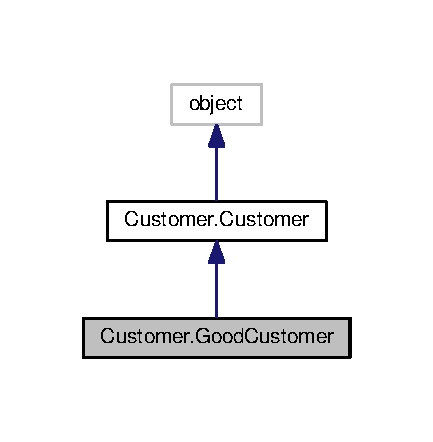
\includegraphics[width=208pt]{class_customer_1_1_good_customer__inherit__graph}
\end{center}
\end{figure}


Collaboration diagram for Customer.\+Good\+Customer\+:\nopagebreak
\begin{figure}[H]
\begin{center}
\leavevmode
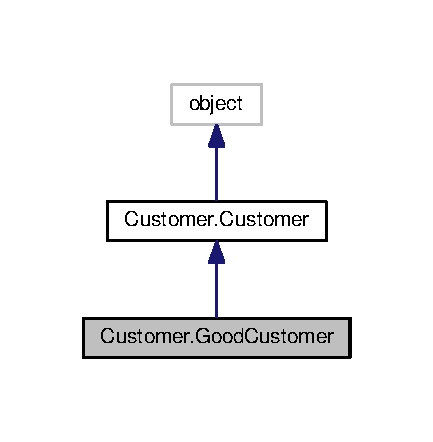
\includegraphics[width=208pt]{class_customer_1_1_good_customer__coll__graph}
\end{center}
\end{figure}
\subsection*{Public Member Functions}
\begin{DoxyCompactItemize}
\item 
\mbox{\Hypertarget{class_customer_1_1_good_customer_a7b3c3a1b2561f3c5481450861283197c}\label{class_customer_1_1_good_customer_a7b3c3a1b2561f3c5481450861283197c}} 
def {\bfseries \+\_\+\+\_\+init\+\_\+\+\_\+} (self)
\item 
\mbox{\Hypertarget{class_customer_1_1_good_customer_a016f60237d8510835f7776f262faf30a}\label{class_customer_1_1_good_customer_a016f60237d8510835f7776f262faf30a}} 
def {\bfseries choose\+\_\+shop} (self, num\+\_\+shops)
\end{DoxyCompactItemize}
\subsection*{Public Attributes}
\begin{DoxyCompactItemize}
\item 
\mbox{\Hypertarget{class_customer_1_1_good_customer_ab81ebccfeb36eb265aa812b49a23815e}\label{class_customer_1_1_good_customer_ab81ebccfeb36eb265aa812b49a23815e}} 
{\bfseries recycle\+\_\+prob}
\item 
\mbox{\Hypertarget{class_customer_1_1_good_customer_af9048444ab878fe7f946229e102b4d4d}\label{class_customer_1_1_good_customer_af9048444ab878fe7f946229e102b4d4d}} 
{\bfseries preferred\+\_\+shop}
\end{DoxyCompactItemize}
\subsection*{Additional Inherited Members}


\subsection{Detailed Description}
\begin{DoxyVerb}A good customer recycles goods with a high probability and always revisits his favorite store
to maximize his reputation.
\end{DoxyVerb}
 

The documentation for this class was generated from the following file\+:\begin{DoxyCompactItemize}
\item 
/home/prash/workspace/dev\+\_\+space/demo\+\_\+apps/\+Reusabili\+Token/\+Reusabili\+Token\+Simulator/src/Customer.\+py\end{DoxyCompactItemize}

\hypertarget{class_customer_1_1_neutral_customer}{}\section{Customer.\+Neutral\+Customer Class Reference}
\label{class_customer_1_1_neutral_customer}\index{Customer.\+Neutral\+Customer@{Customer.\+Neutral\+Customer}}


Inheritance diagram for Customer.\+Neutral\+Customer\+:\nopagebreak
\begin{figure}[H]
\begin{center}
\leavevmode
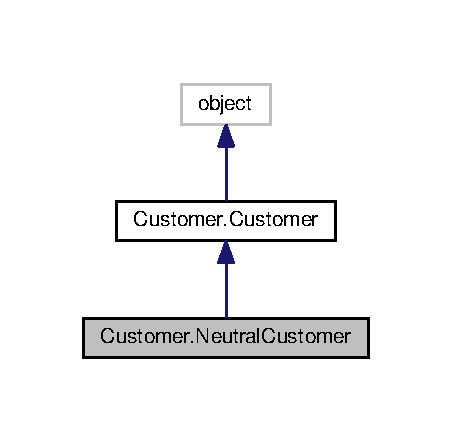
\includegraphics[width=217pt]{class_customer_1_1_neutral_customer__inherit__graph}
\end{center}
\end{figure}


Collaboration diagram for Customer.\+Neutral\+Customer\+:\nopagebreak
\begin{figure}[H]
\begin{center}
\leavevmode
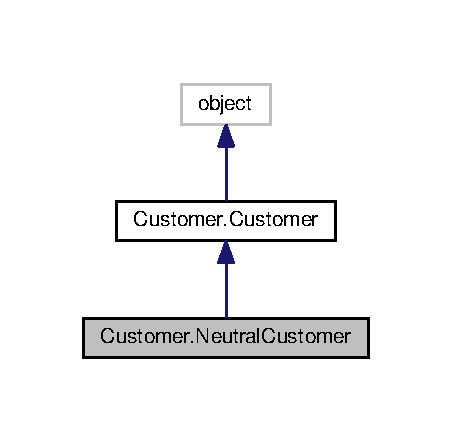
\includegraphics[width=217pt]{class_customer_1_1_neutral_customer__coll__graph}
\end{center}
\end{figure}
\subsection*{Public Member Functions}
\begin{DoxyCompactItemize}
\item 
\mbox{\Hypertarget{class_customer_1_1_neutral_customer_a17dfe793e750ec44daad18fadf64bb76}\label{class_customer_1_1_neutral_customer_a17dfe793e750ec44daad18fadf64bb76}} 
def {\bfseries \+\_\+\+\_\+init\+\_\+\+\_\+} (self)
\item 
\mbox{\Hypertarget{class_customer_1_1_neutral_customer_a24af596788db64a679ea26ced7e1664b}\label{class_customer_1_1_neutral_customer_a24af596788db64a679ea26ced7e1664b}} 
def {\bfseries choose\+\_\+shop} (self, num\+\_\+shops)
\end{DoxyCompactItemize}
\subsection*{Public Attributes}
\begin{DoxyCompactItemize}
\item 
\mbox{\Hypertarget{class_customer_1_1_neutral_customer_a7f16af6df93d1cd9553a787f468642b8}\label{class_customer_1_1_neutral_customer_a7f16af6df93d1cd9553a787f468642b8}} 
{\bfseries recycle\+\_\+prob}
\item 
\mbox{\Hypertarget{class_customer_1_1_neutral_customer_a9b0a639e5346d26c28f1f95f3038d779}\label{class_customer_1_1_neutral_customer_a9b0a639e5346d26c28f1f95f3038d779}} 
{\bfseries preferred\+\_\+shops}
\item 
\mbox{\Hypertarget{class_customer_1_1_neutral_customer_a1aa0d47d29a0d0d00b8f86f88582f6d0}\label{class_customer_1_1_neutral_customer_a1aa0d47d29a0d0d00b8f86f88582f6d0}} 
{\bfseries preference\+\_\+ratio}
\end{DoxyCompactItemize}
\subsection*{Additional Inherited Members}


\subsection{Detailed Description}
\begin{DoxyVerb}A neutral customer recycles his goods with a decent probability and revisits a small subset of all stores
that he likes to visit.
\end{DoxyVerb}
 

The documentation for this class was generated from the following file\+:\begin{DoxyCompactItemize}
\item 
/home/prash/workspace/dev\+\_\+space/demo\+\_\+apps/\+Reusabili\+Token/\+Reusabili\+Token\+Simulator/src/Customer.\+py\end{DoxyCompactItemize}

\hypertarget{class_shop_1_1_shop}{}\section{Shop.\+Shop Class Reference}
\label{class_shop_1_1_shop}\index{Shop.\+Shop@{Shop.\+Shop}}


Inheritance diagram for Shop.\+Shop\+:\nopagebreak
\begin{figure}[H]
\begin{center}
\leavevmode
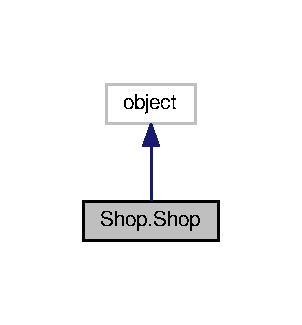
\includegraphics[width=145pt]{class_shop_1_1_shop__inherit__graph}
\end{center}
\end{figure}


Collaboration diagram for Shop.\+Shop\+:\nopagebreak
\begin{figure}[H]
\begin{center}
\leavevmode
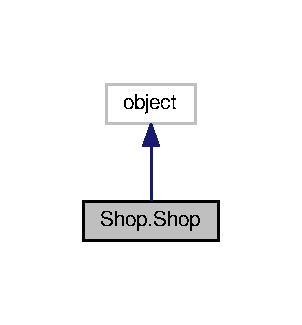
\includegraphics[width=145pt]{class_shop_1_1_shop__coll__graph}
\end{center}
\end{figure}
\subsection*{Public Member Functions}
\begin{DoxyCompactItemize}
\item 
\mbox{\Hypertarget{class_shop_1_1_shop_a307a03fe53eb1c546fdd731386ec85ad}\label{class_shop_1_1_shop_a307a03fe53eb1c546fdd731386ec85ad}} 
def {\bfseries \+\_\+\+\_\+init\+\_\+\+\_\+} (self)
\item 
def \mbox{\hyperlink{class_shop_1_1_shop_a2fc55120d0b88ac30018a14a98632e43}{get\+\_\+shop\+\_\+address}} (self)
\item 
def \mbox{\hyperlink{class_shop_1_1_shop_aa57249095c0d73dcc3bf6223ec15c0ad}{get\+\_\+coin\+\_\+count}} (self)
\item 
def \mbox{\hyperlink{class_shop_1_1_shop_af62739edeb16dfc57c23c5a4ff1a54e9}{buy\+\_\+with\+\_\+coins}} (self, coins)
\item 
def \mbox{\hyperlink{class_shop_1_1_shop_a34e743286fb3f62aef7cf8f9ec242e03}{pay\+\_\+dues\+\_\+to\+\_\+smart\+\_\+contract}} (self, smart\+\_\+contract)
\end{DoxyCompactItemize}
\subsection*{Public Attributes}
\begin{DoxyCompactItemize}
\item 
\mbox{\Hypertarget{class_shop_1_1_shop_aad32dbba8d9f9b0fef32185b90457f18}\label{class_shop_1_1_shop_aad32dbba8d9f9b0fef32185b90457f18}} 
{\bfseries shop\+\_\+id}
\item 
\mbox{\Hypertarget{class_shop_1_1_shop_ad50dfb8118821dc93843241195cdc990}\label{class_shop_1_1_shop_ad50dfb8118821dc93843241195cdc990}} 
{\bfseries name}
\item 
\mbox{\Hypertarget{class_shop_1_1_shop_ab4c935094df2a25f6f7bad4634532db7}\label{class_shop_1_1_shop_ab4c935094df2a25f6f7bad4634532db7}} 
{\bfseries coin\+\_\+count}
\end{DoxyCompactItemize}
\subsection*{Static Public Attributes}
\begin{DoxyCompactItemize}
\item 
\mbox{\Hypertarget{class_shop_1_1_shop_ad0e4a35831e14af289f21c81d1a56261}\label{class_shop_1_1_shop_ad0e4a35831e14af289f21c81d1a56261}} 
int {\bfseries S\+H\+O\+P\+\_\+\+ID} = 0
\end{DoxyCompactItemize}


\subsection{Detailed Description}
\begin{DoxyVerb}This is an implementation of a generic shop that accepts ReusabiliTokens
\end{DoxyVerb}
 

\subsection{Member Function Documentation}
\mbox{\Hypertarget{class_shop_1_1_shop_af62739edeb16dfc57c23c5a4ff1a54e9}\label{class_shop_1_1_shop_af62739edeb16dfc57c23c5a4ff1a54e9}} 
\index{Shop\+::\+Shop@{Shop\+::\+Shop}!buy\+\_\+with\+\_\+coins@{buy\+\_\+with\+\_\+coins}}
\index{buy\+\_\+with\+\_\+coins@{buy\+\_\+with\+\_\+coins}!Shop\+::\+Shop@{Shop\+::\+Shop}}
\subsubsection{\texorpdfstring{buy\+\_\+with\+\_\+coins()}{buy\_with\_coins()}}
{\footnotesize\ttfamily def Shop.\+Shop.\+buy\+\_\+with\+\_\+coins (\begin{DoxyParamCaption}\item[{}]{self,  }\item[{}]{coins }\end{DoxyParamCaption})}

\begin{DoxyVerb}Every time a customer decides to buy with ReusabiliTokens from this shop, the shop
gets that many ReusabiliTokens
:param coins: number of coins that this shop gets
:return: None
\end{DoxyVerb}
 \mbox{\Hypertarget{class_shop_1_1_shop_aa57249095c0d73dcc3bf6223ec15c0ad}\label{class_shop_1_1_shop_aa57249095c0d73dcc3bf6223ec15c0ad}} 
\index{Shop\+::\+Shop@{Shop\+::\+Shop}!get\+\_\+coin\+\_\+count@{get\+\_\+coin\+\_\+count}}
\index{get\+\_\+coin\+\_\+count@{get\+\_\+coin\+\_\+count}!Shop\+::\+Shop@{Shop\+::\+Shop}}
\subsubsection{\texorpdfstring{get\+\_\+coin\+\_\+count()}{get\_coin\_count()}}
{\footnotesize\ttfamily def Shop.\+Shop.\+get\+\_\+coin\+\_\+count (\begin{DoxyParamCaption}\item[{}]{self }\end{DoxyParamCaption})}

\begin{DoxyVerb}Get the number of coins that this shop is in possession of.
:return: coin count of the shop
\end{DoxyVerb}
 \mbox{\Hypertarget{class_shop_1_1_shop_a2fc55120d0b88ac30018a14a98632e43}\label{class_shop_1_1_shop_a2fc55120d0b88ac30018a14a98632e43}} 
\index{Shop\+::\+Shop@{Shop\+::\+Shop}!get\+\_\+shop\+\_\+address@{get\+\_\+shop\+\_\+address}}
\index{get\+\_\+shop\+\_\+address@{get\+\_\+shop\+\_\+address}!Shop\+::\+Shop@{Shop\+::\+Shop}}
\subsubsection{\texorpdfstring{get\+\_\+shop\+\_\+address()}{get\_shop\_address()}}
{\footnotesize\ttfamily def Shop.\+Shop.\+get\+\_\+shop\+\_\+address (\begin{DoxyParamCaption}\item[{}]{self }\end{DoxyParamCaption})}

\begin{DoxyVerb}Get the address of this shop.
:return: shop address
\end{DoxyVerb}
 \mbox{\Hypertarget{class_shop_1_1_shop_a34e743286fb3f62aef7cf8f9ec242e03}\label{class_shop_1_1_shop_a34e743286fb3f62aef7cf8f9ec242e03}} 
\index{Shop\+::\+Shop@{Shop\+::\+Shop}!pay\+\_\+dues\+\_\+to\+\_\+smart\+\_\+contract@{pay\+\_\+dues\+\_\+to\+\_\+smart\+\_\+contract}}
\index{pay\+\_\+dues\+\_\+to\+\_\+smart\+\_\+contract@{pay\+\_\+dues\+\_\+to\+\_\+smart\+\_\+contract}!Shop\+::\+Shop@{Shop\+::\+Shop}}
\subsubsection{\texorpdfstring{pay\+\_\+dues\+\_\+to\+\_\+smart\+\_\+contract()}{pay\_dues\_to\_smart\_contract()}}
{\footnotesize\ttfamily def Shop.\+Shop.\+pay\+\_\+dues\+\_\+to\+\_\+smart\+\_\+contract (\begin{DoxyParamCaption}\item[{}]{self,  }\item[{}]{smart\+\_\+contract }\end{DoxyParamCaption})}

\begin{DoxyVerb}This function makes this shop pay whatever ReusabiliTokens it has to the smart contract.
:param smart_contract: the smart contract to which the payment should be made
:return: None
\end{DoxyVerb}
 

The documentation for this class was generated from the following file\+:\begin{DoxyCompactItemize}
\item 
/home/prash/workspace/dev\+\_\+space/demo\+\_\+apps/\+Reusabili\+Token/\+Reusabili\+Token\+Simulator/src/Shop.\+py\end{DoxyCompactItemize}

\hypertarget{class_shop_list_oracle_1_1_shop_list_oracle}{}\section{Shop\+List\+Oracle.\+Shop\+List\+Oracle Class Reference}
\label{class_shop_list_oracle_1_1_shop_list_oracle}\index{Shop\+List\+Oracle.\+Shop\+List\+Oracle@{Shop\+List\+Oracle.\+Shop\+List\+Oracle}}


Inheritance diagram for Shop\+List\+Oracle.\+Shop\+List\+Oracle\+:\nopagebreak
\begin{figure}[H]
\begin{center}
\leavevmode
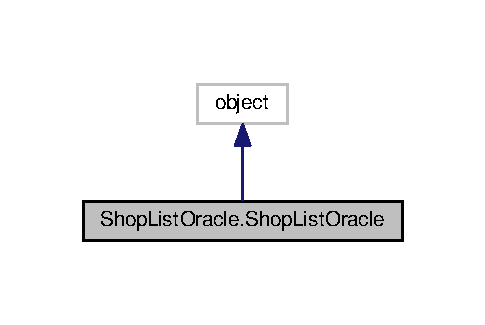
\includegraphics[width=233pt]{class_shop_list_oracle_1_1_shop_list_oracle__inherit__graph}
\end{center}
\end{figure}


Collaboration diagram for Shop\+List\+Oracle.\+Shop\+List\+Oracle\+:\nopagebreak
\begin{figure}[H]
\begin{center}
\leavevmode
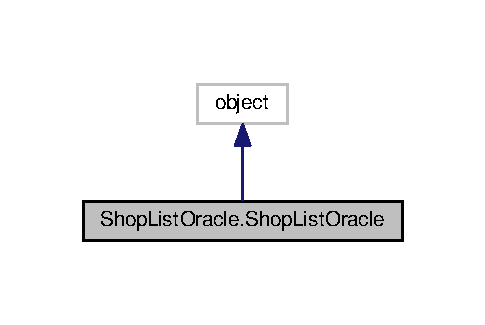
\includegraphics[width=233pt]{class_shop_list_oracle_1_1_shop_list_oracle__coll__graph}
\end{center}
\end{figure}
\subsection*{Public Member Functions}
\begin{DoxyCompactItemize}
\item 
\mbox{\Hypertarget{class_shop_list_oracle_1_1_shop_list_oracle_acf67255437b928eb038f08067297602f}\label{class_shop_list_oracle_1_1_shop_list_oracle_acf67255437b928eb038f08067297602f}} 
def {\bfseries \+\_\+\+\_\+init\+\_\+\+\_\+} (self)
\item 
def \mbox{\hyperlink{class_shop_list_oracle_1_1_shop_list_oracle_a82a22c3a5075c86d96e6e2338840309c}{verify\+\_\+shop}} (self, shop\+\_\+address)
\item 
def \mbox{\hyperlink{class_shop_list_oracle_1_1_shop_list_oracle_a8c1008ee26d4b32dbe8434f08cd5d667}{register\+\_\+new\+\_\+shop}} (self, shop\+\_\+address)
\end{DoxyCompactItemize}
\subsection*{Public Attributes}
\begin{DoxyCompactItemize}
\item 
\mbox{\Hypertarget{class_shop_list_oracle_1_1_shop_list_oracle_a27e95df0f44a65951dd7b8d50deb4654}\label{class_shop_list_oracle_1_1_shop_list_oracle_a27e95df0f44a65951dd7b8d50deb4654}} 
{\bfseries shop\+\_\+list}
\end{DoxyCompactItemize}


\subsection{Detailed Description}
\begin{DoxyVerb}This is an implementation of an Oracle that checks if a specific address belongs
to a registered shop.
\end{DoxyVerb}
 

\subsection{Member Function Documentation}
\mbox{\Hypertarget{class_shop_list_oracle_1_1_shop_list_oracle_a8c1008ee26d4b32dbe8434f08cd5d667}\label{class_shop_list_oracle_1_1_shop_list_oracle_a8c1008ee26d4b32dbe8434f08cd5d667}} 
\index{Shop\+List\+Oracle\+::\+Shop\+List\+Oracle@{Shop\+List\+Oracle\+::\+Shop\+List\+Oracle}!register\+\_\+new\+\_\+shop@{register\+\_\+new\+\_\+shop}}
\index{register\+\_\+new\+\_\+shop@{register\+\_\+new\+\_\+shop}!Shop\+List\+Oracle\+::\+Shop\+List\+Oracle@{Shop\+List\+Oracle\+::\+Shop\+List\+Oracle}}
\subsubsection{\texorpdfstring{register\+\_\+new\+\_\+shop()}{register\_new\_shop()}}
{\footnotesize\ttfamily def Shop\+List\+Oracle.\+Shop\+List\+Oracle.\+register\+\_\+new\+\_\+shop (\begin{DoxyParamCaption}\item[{}]{self,  }\item[{}]{shop\+\_\+address }\end{DoxyParamCaption})}

\begin{DoxyVerb}This function is used to register a new shop with the oracle.
:param shop_address: the address of the shop to register
:return: None
\end{DoxyVerb}
 \mbox{\Hypertarget{class_shop_list_oracle_1_1_shop_list_oracle_a82a22c3a5075c86d96e6e2338840309c}\label{class_shop_list_oracle_1_1_shop_list_oracle_a82a22c3a5075c86d96e6e2338840309c}} 
\index{Shop\+List\+Oracle\+::\+Shop\+List\+Oracle@{Shop\+List\+Oracle\+::\+Shop\+List\+Oracle}!verify\+\_\+shop@{verify\+\_\+shop}}
\index{verify\+\_\+shop@{verify\+\_\+shop}!Shop\+List\+Oracle\+::\+Shop\+List\+Oracle@{Shop\+List\+Oracle\+::\+Shop\+List\+Oracle}}
\subsubsection{\texorpdfstring{verify\+\_\+shop()}{verify\_shop()}}
{\footnotesize\ttfamily def Shop\+List\+Oracle.\+Shop\+List\+Oracle.\+verify\+\_\+shop (\begin{DoxyParamCaption}\item[{}]{self,  }\item[{}]{shop\+\_\+address }\end{DoxyParamCaption})}

\begin{DoxyVerb}The smart contract calls this function to verify if the given address is indeed a shop address
:param shop_address: the address to verify
:return: returns True if the given address is indeed that of a registered shop
\end{DoxyVerb}
 

The documentation for this class was generated from the following file\+:\begin{DoxyCompactItemize}
\item 
/home/prash/workspace/dev\+\_\+space/demo\+\_\+apps/\+Reusabili\+Token/\+Reusabili\+Token\+Simulator/src/Shop\+List\+Oracle.\+py\end{DoxyCompactItemize}

\hypertarget{class_simulation_engine_1_1_simulation_engine}{}\section{Simulation\+Engine.\+Simulation\+Engine Class Reference}
\label{class_simulation_engine_1_1_simulation_engine}\index{Simulation\+Engine.\+Simulation\+Engine@{Simulation\+Engine.\+Simulation\+Engine}}


Inheritance diagram for Simulation\+Engine.\+Simulation\+Engine\+:\nopagebreak
\begin{figure}[H]
\begin{center}
\leavevmode
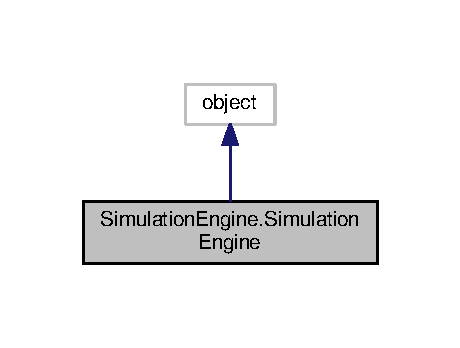
\includegraphics[width=221pt]{class_simulation_engine_1_1_simulation_engine__inherit__graph}
\end{center}
\end{figure}


Collaboration diagram for Simulation\+Engine.\+Simulation\+Engine\+:\nopagebreak
\begin{figure}[H]
\begin{center}
\leavevmode
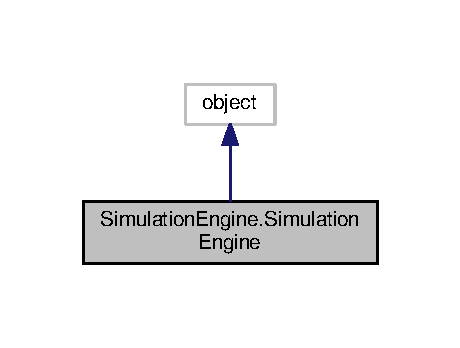
\includegraphics[width=221pt]{class_simulation_engine_1_1_simulation_engine__coll__graph}
\end{center}
\end{figure}
\subsection*{Public Member Functions}
\begin{DoxyCompactItemize}
\item 
def \mbox{\hyperlink{class_simulation_engine_1_1_simulation_engine_adc5d57358f9043ec19d957d6df7afa6e}{\+\_\+\+\_\+init\+\_\+\+\_\+}} (self, num\+\_\+customers, num\+\_\+shops, sim\+\_\+iters, coin\+\_\+limit, rep\+\_\+limit, coin\+\_\+rep\+\_\+factor, payment\+\_\+due)
\item 
def \mbox{\hyperlink{class_simulation_engine_1_1_simulation_engine_a3a741dc8da93469cd400bf8ff198de05}{run}} (self, claim\+\_\+failure\+\_\+probability=0.\+00001)
\end{DoxyCompactItemize}
\subsection*{Public Attributes}
\begin{DoxyCompactItemize}
\item 
\mbox{\Hypertarget{class_simulation_engine_1_1_simulation_engine_a0e2add8e8ec673e61e12c488b7b352a8}\label{class_simulation_engine_1_1_simulation_engine_a0e2add8e8ec673e61e12c488b7b352a8}} 
{\bfseries num\+\_\+customers}
\item 
\mbox{\Hypertarget{class_simulation_engine_1_1_simulation_engine_afa6a33d76f31ef40c7df921c1907bfb5}\label{class_simulation_engine_1_1_simulation_engine_afa6a33d76f31ef40c7df921c1907bfb5}} 
{\bfseries num\+\_\+shops}
\item 
\mbox{\Hypertarget{class_simulation_engine_1_1_simulation_engine_a9b97f9c7a89dcba934ecd6b0ca967dfe}\label{class_simulation_engine_1_1_simulation_engine_a9b97f9c7a89dcba934ecd6b0ca967dfe}} 
{\bfseries sim\+\_\+iters}
\item 
\mbox{\Hypertarget{class_simulation_engine_1_1_simulation_engine_a177034fd34eb202b73e285413cecf12e}\label{class_simulation_engine_1_1_simulation_engine_a177034fd34eb202b73e285413cecf12e}} 
{\bfseries customers}
\item 
\mbox{\Hypertarget{class_simulation_engine_1_1_simulation_engine_a9aa42f2728739dbfa9f4e608070598f0}\label{class_simulation_engine_1_1_simulation_engine_a9aa42f2728739dbfa9f4e608070598f0}} 
{\bfseries shops}
\item 
\mbox{\Hypertarget{class_simulation_engine_1_1_simulation_engine_a3ffa3c62fbf9e1e4c1304988269e082e}\label{class_simulation_engine_1_1_simulation_engine_a3ffa3c62fbf9e1e4c1304988269e082e}} 
{\bfseries time\+\_\+oracle}
\item 
\mbox{\Hypertarget{class_simulation_engine_1_1_simulation_engine_a6679f37621cd193355717789ae122b2f}\label{class_simulation_engine_1_1_simulation_engine_a6679f37621cd193355717789ae122b2f}} 
{\bfseries shop\+\_\+list\+\_\+oracle}
\item 
\mbox{\Hypertarget{class_simulation_engine_1_1_simulation_engine_a9424d8a633bf0d6ce3f44767d4eca542}\label{class_simulation_engine_1_1_simulation_engine_a9424d8a633bf0d6ce3f44767d4eca542}} 
{\bfseries address}
\item 
\mbox{\Hypertarget{class_simulation_engine_1_1_simulation_engine_a129c8525646638a0f5712a83c4c9f8de}\label{class_simulation_engine_1_1_simulation_engine_a129c8525646638a0f5712a83c4c9f8de}} 
{\bfseries smart\+\_\+contract}
\item 
\mbox{\Hypertarget{class_simulation_engine_1_1_simulation_engine_ab58c9ea0ed901c6e224272f56f904ced}\label{class_simulation_engine_1_1_simulation_engine_ab58c9ea0ed901c6e224272f56f904ced}} 
{\bfseries coin\+\_\+limit}
\item 
\mbox{\Hypertarget{class_simulation_engine_1_1_simulation_engine_ac9670ebfef048cce57e6f6390c8d416f}\label{class_simulation_engine_1_1_simulation_engine_ac9670ebfef048cce57e6f6390c8d416f}} 
{\bfseries rep\+\_\+limit}
\item 
\mbox{\Hypertarget{class_simulation_engine_1_1_simulation_engine_a187c2292dd5d87dd7ea606537150cc1f}\label{class_simulation_engine_1_1_simulation_engine_a187c2292dd5d87dd7ea606537150cc1f}} 
{\bfseries payment\+\_\+due}
\item 
\mbox{\Hypertarget{class_simulation_engine_1_1_simulation_engine_a32c23fec3a8437741542742f0e63d53b}\label{class_simulation_engine_1_1_simulation_engine_a32c23fec3a8437741542742f0e63d53b}} 
{\bfseries coin\+\_\+rep\+\_\+factor}
\end{DoxyCompactItemize}


\subsection{Detailed Description}
\begin{DoxyVerb}This is the engine that runs the market simulation
\end{DoxyVerb}
 

\subsection{Constructor \& Destructor Documentation}
\mbox{\Hypertarget{class_simulation_engine_1_1_simulation_engine_adc5d57358f9043ec19d957d6df7afa6e}\label{class_simulation_engine_1_1_simulation_engine_adc5d57358f9043ec19d957d6df7afa6e}} 
\index{Simulation\+Engine\+::\+Simulation\+Engine@{Simulation\+Engine\+::\+Simulation\+Engine}!\+\_\+\+\_\+init\+\_\+\+\_\+@{\+\_\+\+\_\+init\+\_\+\+\_\+}}
\index{\+\_\+\+\_\+init\+\_\+\+\_\+@{\+\_\+\+\_\+init\+\_\+\+\_\+}!Simulation\+Engine\+::\+Simulation\+Engine@{Simulation\+Engine\+::\+Simulation\+Engine}}
\subsubsection{\texorpdfstring{\+\_\+\+\_\+init\+\_\+\+\_\+()}{\_\_init\_\_()}}
{\footnotesize\ttfamily def Simulation\+Engine.\+Simulation\+Engine.\+\_\+\+\_\+init\+\_\+\+\_\+ (\begin{DoxyParamCaption}\item[{}]{self,  }\item[{}]{num\+\_\+customers,  }\item[{}]{num\+\_\+shops,  }\item[{}]{sim\+\_\+iters,  }\item[{}]{coin\+\_\+limit,  }\item[{}]{rep\+\_\+limit,  }\item[{}]{coin\+\_\+rep\+\_\+factor,  }\item[{}]{payment\+\_\+due }\end{DoxyParamCaption})}

\begin{DoxyVerb}Constructor
:param num_customers: the number of customers in the market
:param num_shops: the number of shops in the market
:param sim_iters: the number of iterations to simulate the market
:param coin_limit: the maximum coin that a customer can possess (NOT USED CURRENTLY)
:param rep_limit: the maximum reputation that a customer can earn
:param coin_rep_factor: a multiplicative factor to convert reputations to ReusabiliTokens
:param payment_due: the duration over which shops have to pay back their dues
\end{DoxyVerb}
 

\subsection{Member Function Documentation}
\mbox{\Hypertarget{class_simulation_engine_1_1_simulation_engine_a3a741dc8da93469cd400bf8ff198de05}\label{class_simulation_engine_1_1_simulation_engine_a3a741dc8da93469cd400bf8ff198de05}} 
\index{Simulation\+Engine\+::\+Simulation\+Engine@{Simulation\+Engine\+::\+Simulation\+Engine}!run@{run}}
\index{run@{run}!Simulation\+Engine\+::\+Simulation\+Engine@{Simulation\+Engine\+::\+Simulation\+Engine}}
\subsubsection{\texorpdfstring{run()}{run()}}
{\footnotesize\ttfamily def Simulation\+Engine.\+Simulation\+Engine.\+run (\begin{DoxyParamCaption}\item[{}]{self,  }\item[{}]{claim\+\_\+failure\+\_\+probability = {\ttfamily 0.00001} }\end{DoxyParamCaption})}

\begin{DoxyVerb}Run the simulator
:param claim_failure_probability: probability of a customer claim being false
:return: None
\end{DoxyVerb}
 

The documentation for this class was generated from the following file\+:\begin{DoxyCompactItemize}
\item 
/home/prash/workspace/dev\+\_\+space/demo\+\_\+apps/\+Reusabili\+Token/\+Reusabili\+Token\+Simulator/src/Simulation\+Engine.\+py\end{DoxyCompactItemize}

\hypertarget{class_simulation_time_oracle_1_1_simulation_time_oracle}{}\section{Simulation\+Time\+Oracle.\+Simulation\+Time\+Oracle Class Reference}
\label{class_simulation_time_oracle_1_1_simulation_time_oracle}\index{Simulation\+Time\+Oracle.\+Simulation\+Time\+Oracle@{Simulation\+Time\+Oracle.\+Simulation\+Time\+Oracle}}


Inheritance diagram for Simulation\+Time\+Oracle.\+Simulation\+Time\+Oracle\+:\nopagebreak
\begin{figure}[H]
\begin{center}
\leavevmode
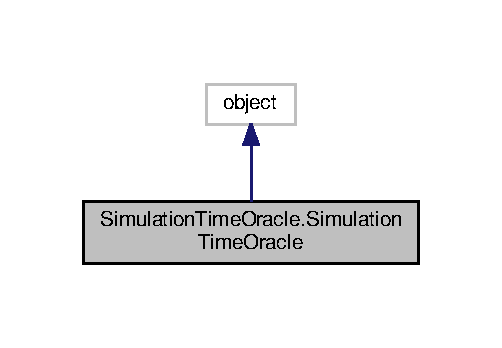
\includegraphics[width=241pt]{class_simulation_time_oracle_1_1_simulation_time_oracle__inherit__graph}
\end{center}
\end{figure}


Collaboration diagram for Simulation\+Time\+Oracle.\+Simulation\+Time\+Oracle\+:\nopagebreak
\begin{figure}[H]
\begin{center}
\leavevmode
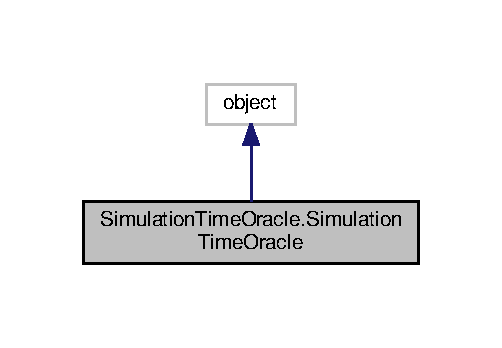
\includegraphics[width=241pt]{class_simulation_time_oracle_1_1_simulation_time_oracle__coll__graph}
\end{center}
\end{figure}
\subsection*{Public Member Functions}
\begin{DoxyCompactItemize}
\item 
\mbox{\Hypertarget{class_simulation_time_oracle_1_1_simulation_time_oracle_a6295da8dc38378a67d5db534e20d6426}\label{class_simulation_time_oracle_1_1_simulation_time_oracle_a6295da8dc38378a67d5db534e20d6426}} 
def {\bfseries \+\_\+\+\_\+init\+\_\+\+\_\+} (self)
\item 
def \mbox{\hyperlink{class_simulation_time_oracle_1_1_simulation_time_oracle_a2a89702650ee07d32b369da6eae552b9}{increment\+\_\+time}} (self)
\item 
def \mbox{\hyperlink{class_simulation_time_oracle_1_1_simulation_time_oracle_ad567bc0e28a99369aaa448370c9a1944}{get\+\_\+time}} (self)
\end{DoxyCompactItemize}
\subsection*{Public Attributes}
\begin{DoxyCompactItemize}
\item 
\mbox{\Hypertarget{class_simulation_time_oracle_1_1_simulation_time_oracle_a9ec52d33610ad7fcdb3370017b13277a}\label{class_simulation_time_oracle_1_1_simulation_time_oracle_a9ec52d33610ad7fcdb3370017b13277a}} 
{\bfseries time}
\end{DoxyCompactItemize}


\subsection{Detailed Description}
\begin{DoxyVerb}An oracle that gives the True time
\end{DoxyVerb}
 

\subsection{Member Function Documentation}
\mbox{\Hypertarget{class_simulation_time_oracle_1_1_simulation_time_oracle_ad567bc0e28a99369aaa448370c9a1944}\label{class_simulation_time_oracle_1_1_simulation_time_oracle_ad567bc0e28a99369aaa448370c9a1944}} 
\index{Simulation\+Time\+Oracle\+::\+Simulation\+Time\+Oracle@{Simulation\+Time\+Oracle\+::\+Simulation\+Time\+Oracle}!get\+\_\+time@{get\+\_\+time}}
\index{get\+\_\+time@{get\+\_\+time}!Simulation\+Time\+Oracle\+::\+Simulation\+Time\+Oracle@{Simulation\+Time\+Oracle\+::\+Simulation\+Time\+Oracle}}
\subsubsection{\texorpdfstring{get\+\_\+time()}{get\_time()}}
{\footnotesize\ttfamily def Simulation\+Time\+Oracle.\+Simulation\+Time\+Oracle.\+get\+\_\+time (\begin{DoxyParamCaption}\item[{}]{self }\end{DoxyParamCaption})}

\begin{DoxyVerb}A smart contract would call this function on the oracle to determine some standard wall clock
time
:return: False
\end{DoxyVerb}
 \mbox{\Hypertarget{class_simulation_time_oracle_1_1_simulation_time_oracle_a2a89702650ee07d32b369da6eae552b9}\label{class_simulation_time_oracle_1_1_simulation_time_oracle_a2a89702650ee07d32b369da6eae552b9}} 
\index{Simulation\+Time\+Oracle\+::\+Simulation\+Time\+Oracle@{Simulation\+Time\+Oracle\+::\+Simulation\+Time\+Oracle}!increment\+\_\+time@{increment\+\_\+time}}
\index{increment\+\_\+time@{increment\+\_\+time}!Simulation\+Time\+Oracle\+::\+Simulation\+Time\+Oracle@{Simulation\+Time\+Oracle\+::\+Simulation\+Time\+Oracle}}
\subsubsection{\texorpdfstring{increment\+\_\+time()}{increment\_time()}}
{\footnotesize\ttfamily def Simulation\+Time\+Oracle.\+Simulation\+Time\+Oracle.\+increment\+\_\+time (\begin{DoxyParamCaption}\item[{}]{self }\end{DoxyParamCaption})}

\begin{DoxyVerb}Increment the wall clock time on the Oracle
:return:
\end{DoxyVerb}
 

The documentation for this class was generated from the following file\+:\begin{DoxyCompactItemize}
\item 
/home/prash/workspace/dev\+\_\+space/demo\+\_\+apps/\+Reusabili\+Token/\+Reusabili\+Token\+Simulator/src/Simulation\+Time\+Oracle.\+py\end{DoxyCompactItemize}

\hypertarget{class_smart_contract_1_1_smart_contract}{}\section{Smart\+Contract.\+Smart\+Contract Class Reference}
\label{class_smart_contract_1_1_smart_contract}\index{Smart\+Contract.\+Smart\+Contract@{Smart\+Contract.\+Smart\+Contract}}


Inheritance diagram for Smart\+Contract.\+Smart\+Contract\+:\nopagebreak
\begin{figure}[H]
\begin{center}
\leavevmode
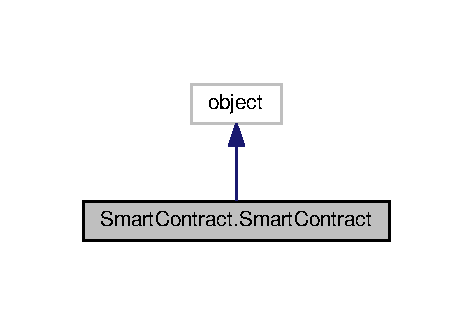
\includegraphics[width=227pt]{class_smart_contract_1_1_smart_contract__inherit__graph}
\end{center}
\end{figure}


Collaboration diagram for Smart\+Contract.\+Smart\+Contract\+:\nopagebreak
\begin{figure}[H]
\begin{center}
\leavevmode
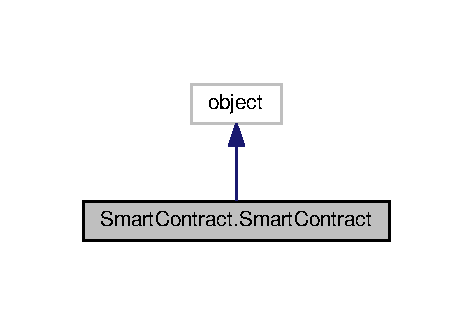
\includegraphics[width=227pt]{class_smart_contract_1_1_smart_contract__coll__graph}
\end{center}
\end{figure}
\subsection*{Public Member Functions}
\begin{DoxyCompactItemize}
\item 
\mbox{\Hypertarget{class_smart_contract_1_1_smart_contract_ae0684adf8d361d2cb2ab0f3e915956c9}\label{class_smart_contract_1_1_smart_contract_ae0684adf8d361d2cb2ab0f3e915956c9}} 
def {\bfseries \+\_\+\+\_\+init\+\_\+\+\_\+} (self, owner\+\_\+address)
\item 
\mbox{\Hypertarget{class_smart_contract_1_1_smart_contract_a1d9defa78b63a8f0aa1bee8dced6df03}\label{class_smart_contract_1_1_smart_contract_a1d9defa78b63a8f0aa1bee8dced6df03}} 
def {\bfseries set\+\_\+oracle} (self, sender\+\_\+address, shop\+\_\+oracle, time\+\_\+oracle)
\item 
\mbox{\Hypertarget{class_smart_contract_1_1_smart_contract_a654ecc9286669fd414850ae961ab0e3a}\label{class_smart_contract_1_1_smart_contract_a654ecc9286669fd414850ae961ab0e3a}} 
def {\bfseries set\+\_\+coin\+\_\+limit} (self, sender\+\_\+address, coin\+\_\+limit)
\item 
\mbox{\Hypertarget{class_smart_contract_1_1_smart_contract_ad5f5a707acec0876eefca40a7094af10}\label{class_smart_contract_1_1_smart_contract_ad5f5a707acec0876eefca40a7094af10}} 
def {\bfseries set\+\_\+reputation\+\_\+limit} (self, sender\+\_\+address, reputation\+\_\+limit)
\item 
\mbox{\Hypertarget{class_smart_contract_1_1_smart_contract_ac6c47b1b975447866a59d16d92fe882e}\label{class_smart_contract_1_1_smart_contract_ac6c47b1b975447866a59d16d92fe882e}} 
def {\bfseries set\+\_\+coins\+\_\+per\+\_\+reputation\+\_\+token} (self, sender\+\_\+address, factor)
\item 
\mbox{\Hypertarget{class_smart_contract_1_1_smart_contract_adc1c69e80e6e11fde584bbcd37284f85}\label{class_smart_contract_1_1_smart_contract_adc1c69e80e6e11fde584bbcd37284f85}} 
def {\bfseries set\+\_\+payment\+\_\+duration} (self, sender\+\_\+address, duration)
\item 
\mbox{\Hypertarget{class_smart_contract_1_1_smart_contract_aacb8fa6992072fdf90415fda78a66148}\label{class_smart_contract_1_1_smart_contract_aacb8fa6992072fdf90415fda78a66148}} 
def {\bfseries check\+\_\+payments} (self, sender\+\_\+address, current\+\_\+time)
\item 
\mbox{\Hypertarget{class_smart_contract_1_1_smart_contract_a7630d7053219be5ff175701637523e1a}\label{class_smart_contract_1_1_smart_contract_a7630d7053219be5ff175701637523e1a}} 
def {\bfseries make\+\_\+payment} (self, shop\+\_\+address, payment)
\item 
\mbox{\Hypertarget{class_smart_contract_1_1_smart_contract_a999674af0040edc43ca9a1162c6826c9}\label{class_smart_contract_1_1_smart_contract_a999674af0040edc43ca9a1162c6826c9}} 
def {\bfseries make\+\_\+claim} (self, shop\+\_\+address, customer\+\_\+address)
\item 
\mbox{\Hypertarget{class_smart_contract_1_1_smart_contract_a0b3ef2dc581778b62b114a18a6ecf425}\label{class_smart_contract_1_1_smart_contract_a0b3ef2dc581778b62b114a18a6ecf425}} 
def {\bfseries verify\+\_\+claim} (self, shop\+\_\+address, customer\+\_\+address)
\item 
\mbox{\Hypertarget{class_smart_contract_1_1_smart_contract_a80b5a9c6340aaca1a057fb5cf35aaab7}\label{class_smart_contract_1_1_smart_contract_a80b5a9c6340aaca1a057fb5cf35aaab7}} 
def {\bfseries customer\+\_\+buys\+\_\+with\+\_\+coin} (self, customer\+\_\+address, shop\+\_\+address, num\+\_\+coins)
\item 
\mbox{\Hypertarget{class_smart_contract_1_1_smart_contract_a1a93d7800c0da5e4a55a274005bbe88f}\label{class_smart_contract_1_1_smart_contract_a1a93d7800c0da5e4a55a274005bbe88f}} 
def {\bfseries deteriorate\+\_\+customer\+\_\+reputation} (self, sender\+\_\+address, value=0.\+05)
\item 
\mbox{\Hypertarget{class_smart_contract_1_1_smart_contract_a1a1470aa88eeac677349edfd34fab0f6}\label{class_smart_contract_1_1_smart_contract_a1a1470aa88eeac677349edfd34fab0f6}} 
def {\bfseries calculate\+\_\+shop\+\_\+reputation} (self, shop\+\_\+address)
\item 
\mbox{\Hypertarget{class_smart_contract_1_1_smart_contract_a049d23b4a18583bacebd00c52b724897}\label{class_smart_contract_1_1_smart_contract_a049d23b4a18583bacebd00c52b724897}} 
def {\bfseries calculate\+\_\+customer\+\_\+reputation} (self, customer\+\_\+address)
\item 
\mbox{\Hypertarget{class_smart_contract_1_1_smart_contract_a6a005188fa4f408363018d54a0db276c}\label{class_smart_contract_1_1_smart_contract_a6a005188fa4f408363018d54a0db276c}} 
def {\bfseries valid\+\_\+shops\+\_\+left} (self, shop\+\_\+addresses)
\item 
\mbox{\Hypertarget{class_smart_contract_1_1_smart_contract_a91f5537dbb6289e0232f9ebab8452c39}\label{class_smart_contract_1_1_smart_contract_a91f5537dbb6289e0232f9ebab8452c39}} 
def {\bfseries get\+\_\+coin\+\_\+map} (self)
\item 
\mbox{\Hypertarget{class_smart_contract_1_1_smart_contract_adc4fc84cb0886588520ba2c5b8ed9d99}\label{class_smart_contract_1_1_smart_contract_adc4fc84cb0886588520ba2c5b8ed9d99}} 
def {\bfseries get\+\_\+reputation\+\_\+map} (self)
\item 
\mbox{\Hypertarget{class_smart_contract_1_1_smart_contract_ae6470553cb9e3db19765805689c05c7c}\label{class_smart_contract_1_1_smart_contract_ae6470553cb9e3db19765805689c05c7c}} 
def {\bfseries get\+\_\+coin\+\_\+purchase\+\_\+map} (self)
\end{DoxyCompactItemize}
\subsection*{Public Attributes}
\begin{DoxyCompactItemize}
\item 
\mbox{\Hypertarget{class_smart_contract_1_1_smart_contract_ac211989cc77f6eceba622bb94faa954b}\label{class_smart_contract_1_1_smart_contract_ac211989cc77f6eceba622bb94faa954b}} 
{\bfseries coin\+\_\+map}
\item 
\mbox{\Hypertarget{class_smart_contract_1_1_smart_contract_a3a64395dba778d06c3ce6e2a3826faad}\label{class_smart_contract_1_1_smart_contract_a3a64395dba778d06c3ce6e2a3826faad}} 
{\bfseries reputation\+\_\+map}
\item 
\mbox{\Hypertarget{class_smart_contract_1_1_smart_contract_aae890929800afe9d33a9cae880aab201}\label{class_smart_contract_1_1_smart_contract_aae890929800afe9d33a9cae880aab201}} 
{\bfseries customer\+\_\+recycle\+\_\+map}
\item 
\mbox{\Hypertarget{class_smart_contract_1_1_smart_contract_a11c156beda2fd1112ef3a8714d9e61de}\label{class_smart_contract_1_1_smart_contract_a11c156beda2fd1112ef3a8714d9e61de}} 
{\bfseries shop\+\_\+coin\+\_\+map}
\item 
\mbox{\Hypertarget{class_smart_contract_1_1_smart_contract_ab094c06e8bc41bf9107a6159f95af492}\label{class_smart_contract_1_1_smart_contract_ab094c06e8bc41bf9107a6159f95af492}} 
{\bfseries cus\+\_\+buys\+\_\+with\+\_\+coin\+\_\+map}
\item 
\mbox{\Hypertarget{class_smart_contract_1_1_smart_contract_ad652d398621ee972abe1c74a04d5bc03}\label{class_smart_contract_1_1_smart_contract_ad652d398621ee972abe1c74a04d5bc03}} 
{\bfseries status}
\item 
\mbox{\Hypertarget{class_smart_contract_1_1_smart_contract_a543fad86dd166d9e29567c0424508a52}\label{class_smart_contract_1_1_smart_contract_a543fad86dd166d9e29567c0424508a52}} 
{\bfseries current\+\_\+customer\+\_\+address}
\item 
\mbox{\Hypertarget{class_smart_contract_1_1_smart_contract_acd90c786485aa072c5b4e96dd7fa3505}\label{class_smart_contract_1_1_smart_contract_acd90c786485aa072c5b4e96dd7fa3505}} 
{\bfseries current\+\_\+shop\+\_\+address}
\item 
\mbox{\Hypertarget{class_smart_contract_1_1_smart_contract_ae1485b34bfa84375c9ba0a0ad12c5435}\label{class_smart_contract_1_1_smart_contract_ae1485b34bfa84375c9ba0a0ad12c5435}} 
{\bfseries owner\+\_\+address}
\item 
\mbox{\Hypertarget{class_smart_contract_1_1_smart_contract_a853b82ee28145c31bc84edfb49d8f738}\label{class_smart_contract_1_1_smart_contract_a853b82ee28145c31bc84edfb49d8f738}} 
{\bfseries shop\+\_\+oracle}
\item 
\mbox{\Hypertarget{class_smart_contract_1_1_smart_contract_a626920b945f3db381cebfd954841cf53}\label{class_smart_contract_1_1_smart_contract_a626920b945f3db381cebfd954841cf53}} 
{\bfseries time\+\_\+oracle}
\item 
\mbox{\Hypertarget{class_smart_contract_1_1_smart_contract_ae0e02f2e9cc6a545af44c991ea1733f2}\label{class_smart_contract_1_1_smart_contract_ae0e02f2e9cc6a545af44c991ea1733f2}} 
{\bfseries known\+\_\+shops}
\item 
\mbox{\Hypertarget{class_smart_contract_1_1_smart_contract_acf3c38cefa3e90afea71f95d52256abf}\label{class_smart_contract_1_1_smart_contract_acf3c38cefa3e90afea71f95d52256abf}} 
{\bfseries black\+\_\+listed\+\_\+shops}
\item 
\mbox{\Hypertarget{class_smart_contract_1_1_smart_contract_a9a909027ab1003841affa9ecefc1932b}\label{class_smart_contract_1_1_smart_contract_a9a909027ab1003841affa9ecefc1932b}} 
{\bfseries shop\+\_\+payment\+\_\+times}
\item 
\mbox{\Hypertarget{class_smart_contract_1_1_smart_contract_aeef5c2db8e7e5a28a0240920df945ac9}\label{class_smart_contract_1_1_smart_contract_aeef5c2db8e7e5a28a0240920df945ac9}} 
{\bfseries reputation\+\_\+limit}
\item 
\mbox{\Hypertarget{class_smart_contract_1_1_smart_contract_a74af331bec11a97e791160cd7062c930}\label{class_smart_contract_1_1_smart_contract_a74af331bec11a97e791160cd7062c930}} 
{\bfseries coin\+\_\+limit}
\item 
\mbox{\Hypertarget{class_smart_contract_1_1_smart_contract_a250470e354f6452ef45f3b28f45eb839}\label{class_smart_contract_1_1_smart_contract_a250470e354f6452ef45f3b28f45eb839}} 
{\bfseries coins\+\_\+per\+\_\+reputation\+\_\+token}
\item 
\mbox{\Hypertarget{class_smart_contract_1_1_smart_contract_a499c8ec7d970a801486ad62b5b422973}\label{class_smart_contract_1_1_smart_contract_a499c8ec7d970a801486ad62b5b422973}} 
{\bfseries payment\+\_\+due\+\_\+date}
\end{DoxyCompactItemize}


The documentation for this class was generated from the following file\+:\begin{DoxyCompactItemize}
\item 
/home/prash/workspace/dev\+\_\+space/demo\+\_\+apps/\+Reusabili\+Token/\+Reusabili\+Token\+Simulator/src/Smart\+Contract.\+py\end{DoxyCompactItemize}

%--- End generated contents ---

% Index
\backmatter
\newpage
\phantomsection
\clearemptydoublepage
\addcontentsline{toc}{chapter}{Index}
\printindex

\end{document}
